
\chapter{Single top quark production with a photon in the Standard Model}
\label{chap:tqgamma_production}
\section{A brief overview of the Standard Model}

The Standard Model (SM) of particle physics, a quantum field theory,  describes today's best theory of particle physics. 
In the SM, there are different kinds of elementary particles and three fundamental forces of nature: the electromagnetic force, the strong force and the weak force. 
Every force coincides with an elementary particle, called a boson, that acts as a mediator of the interaction. Another group of particles are called the fermions, and they only interact with these bosons if they have specific quantities, which are represented by their quantum numbers.

The fermions have spin $s = \frac{1}{2}$ and can be divided into two separate groups. The first group, named quarks, are colour charge carrying fermions. 
There are three up-type quarks (up, strange and top) with an electric charge of $q = +\frac{2}{3}e$ and three down-type quarks (down, charm and bottom) with an electric charge of $q = -\frac{1}{3}e$. 
The second group are the leptons. Three leptons (electron, muon and tau) have an electric charge of $q = +1e$. Furthermore, each of these leptons has a corresponding uncharged lepton partner called a neutrino.
Three different families further categorize leptons and quarks. These quark and lepton families are ordered by mass and consist of an up-type quark, the corresponding down-type quark, a lepton and the corresponding neutrino. 
There is an anti-matter particle equivalent for all fermions where every charge-like quantum number has the opposite sign. 

Particles with integer spin are called bosons. The first group of bosons, gauge bosons with spin $s = 1$, mediate the three fundamental forces. The gauge bosons with spin $s = 1$ are: $gluons$ $g$, $photons$ $\gamma$, $Z$ and $W^{\pm}$. The Higgs boson $H$ is the only boson with spin $s=0$.

Gluons are colour charged and mediate the strong force between colour charged particles, including themselves. The six colour charges are $red$,$green$,$blue$ and their anticolour counterpart. The strong force draws particles with colour together until a colour neutral state is achieved. This can occur when one quark bonds with a quark of the opposite colour, forming a meson. It can also occur when three quarks with $red$, $green$, $blue$ colour charges respectively together form the colour neutral Baryon. 
The strong force becomes stronger the further quarks are repelled from the colour neutral state. If quarks get repelled for a sufficiently high distance, two new quarks are formed, which then bond with the repelled. This process is called colour confinement and can occur many times in a row for higher energies, forming a shower of mesons and baryons. 
Photons mediate the electromagnetic (EM) between electrically charged particles. The massive bosons, $Z$ and $W^{-}$ as well as $W^{+}$ mediate the weak force. The weak force only acts on left-handed particles (and right-handed antiparticles). Here, left-handedness means that the spin direction is opposite to the direction of the momentum of the particle. Right-handed particles have their spin and momentum pointing at the same direction. 
The $W^{\pm}$ bosons are electrically charged, $q = \pm 1e$, and change the flavour of a quark when coupling to it. The flavour refers to the species of a fermion. 
 
The Higgs boson arises from the electroweak theory. The Higgs mechanism provides an explanation for the presence of massive leptons and bosons by breaking the electroweak symmetry. The fermions acquire their mass by coupling with the Higgs boson via the so-called Yukawa interaction.
Before the breaking of the electroweak symmetry, the gauge bosons exist as the electroweak eigenstates $W^1$, $W^2$, $W^3$ and $B$. The breaking of this symmetry mixes $W^3$ and $B$ into the mass eigenstates $Z$ and $\gamma$. 
The eigenstates $W^1$ and $W^2$ mix into the massive eigenstates $W^+$ and $W^-$. 

An overview of the elementary particles in the Standard Model is given in figure \ref{fig:standard_model}.

\begin{figure}
    \centering
    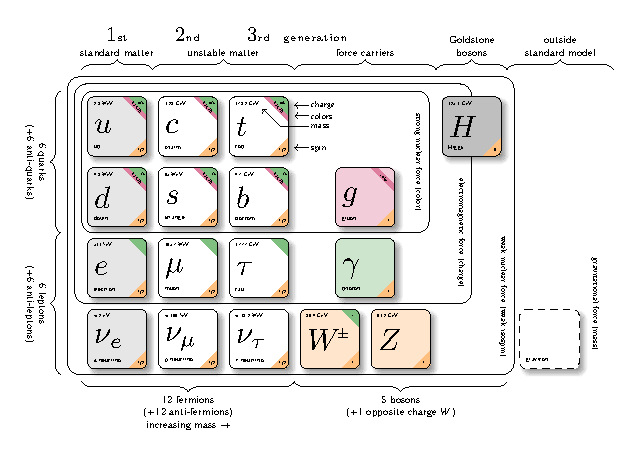
\includegraphics[width=0.9\textwidth]{Plots/model-physics.pdf}
    \caption{Elementary particles of the Standard Model alongside their properties \cite{sm_table}.}
    \label{fig:standard_model}
\end{figure}

\section{The \texorpdfstring{$tq\gamma$}{tqGamma} process in the Standard Model}


The top quark is an up-type quark and the most massive quark of the Standard Model with a mass of $m_t = 173.76 \pm 0.3 \,\si{\giga\electronvolt} (S =1.2)$ \cite{pdg}. Additionally, the top quark has a very small decay width of $\Gamma = 1.42^{+0.19}_{-0.15} \,\si{\giga\electronvolt} (S=1.4)$ \cite{pdg} because of its high mass.
This is one reason why the top quarks unlikely to build any bound states and always decay shortly after production. Only their decay products are observable and can be retraced back to the top quark. 

Top quarks can be produced in three different channels: In the $t$-channel ($tq$), where a single top quark is produced when a bottom quark exchanges a $W$-boson with another quark, the $s$-channel ($tb$), where the top quarks are produced in top-antitop-pairs, and the $tW$-channel, where a gluon and a bottom couple and then decay into a single top and a $W$ boson. In this thesis, the focus lies primarily on the $t$-channel production of the top quark. 
The top quark was first discovered in pair production at the Tevatron in 1995 during a proton-antiproton collision experiment (CITE). In 2009, the D0 \cite{singletop1} and CDF \cite{singletop2} collaborations also separately confirmed the observation of the $t$-channel top quark production at the Tevatron. The combined results are available in reference \cite{singletop3}. 
The CMS experiment at the Large Hadron Collider (LHC) of CERN \cite{CMS} reported evidence for the $t$-channel single production of top quarks in association with a photon ($tq\gamma$) with a significance corresponding to $\sigma = 4.4$. The fiducial cross section 
was measured to be $\sigma(pp\rightarrow tq\gamma)(t\rightarrow\mu \nu b) = 115 \pm 17 (stat) \pm 30 (syst) \,\si{\femto\barn}$ for the photon transverse momentum $p_T^\gamma > 25 \,\si{\giga\electronvolt}$ \ref{PhysRevLett.121.221802}. 

For this thesis, the $tq\gamma$-events are produced in proton-proton-collisoins inside the ATLAS experiment. The ATLAS is discussed in detail in chapter \ref{chap:measurement}. The production of processes in this experiment occurs with elementary particles inside of the protons, called partons. For the production of the $tq\gamma$-process, one gluon provided by the protons may produce a bottom-antibottom-quark pair. The bottom quark may then exchange a $W$-boson with a quark, turning the bottom quark into a top quark and changing the flavour of the quark. This top quark may then radiate a photon. 
It is essential to mention that while this thesis focuses on the top-photon vertex, the photon can be radiated from any charged particle elsewhere in the process. For instance, the bottom quark after the decay of the top may produce a photon.
Afterwards, the top quark decays decays into a $W^+$-boson and a bottom quark. The $W^+$-boson then decays either into an antilepton and neutrino pair or a quark-antiquark pair of opposite quark types. However, only the leptonic decay mode is considered in this thesis.

In Figure \ref{fig:feyn_tqGamma} the leading order Feynman diagram for the $tq\gamma$ production is depicted. The charge conjugated diagram is not shown, but also considered in this thesis.
\begin{figure}
    \centering
    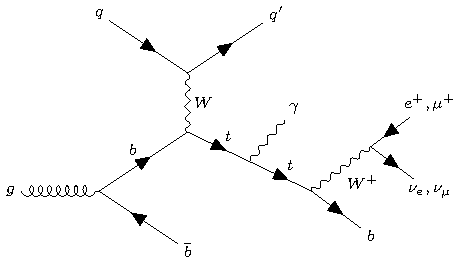
\includegraphics[width=0.6\textwidth]{Plots/s4_feyn_nom.pdf}
    \caption{Leading order Feynman diagram of the $tq\gamma$ process in the Standard Model.}
    \label{fig:feyn_tqGamma}
\end{figure}